\experiment{6}{%
    Plot the distribution of a dataset and examine whether it follows a normal (bell-shaped) curve. Interpret the characteristics of the curve.
}

\subsection{Ploting the distribution}

\subsubsection*{i) Marks}

\begin{lstlisting}[style=python]
import pandas as pd 
import seaborn as sns

df_student = pd.read_csv("dataset.csv", delimiter=',', header='infer')

sns.histplot(df_student['Marks'], kde=True, bins=6)
\end{lstlisting}

\textbf{Output:}

\begin{figure}[H]
    % \centering
    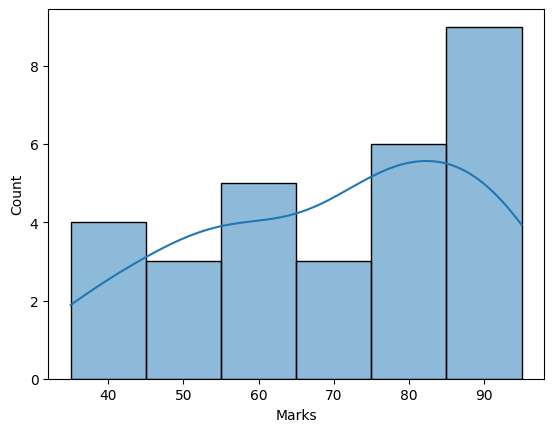
\includegraphics[width=0.75\textwidth]{img/exp6_markHist.png}
    % \caption{Marks of Each Student — Bar Chart}
    % \label{fig:marks_bar}
\end{figure}

\subsubsection*{ii) Study Hours}

\begin{lstlisting}[style=python]
sns.histplot(df_student['StudyHours'], kde=True, bins=6)
\end{lstlisting}

\textbf{Output:}

\begin{figure}[H]
    % \centering
    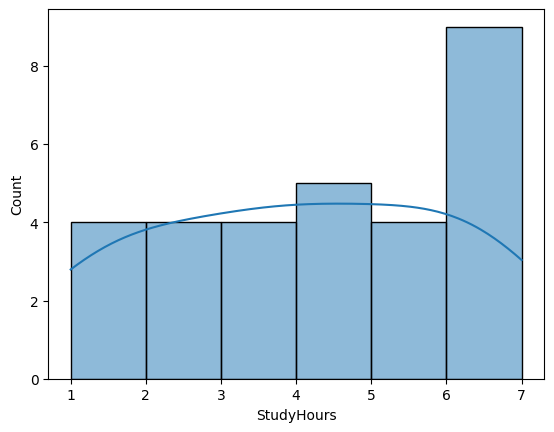
\includegraphics[width=0.75\textwidth]{img/exp6_studyhHist.png}
    % \caption{Marks of Each Student — Bar Chart}
    % \label{fig:marks_bar}
\end{figure}


\subsubsection*{iii) Attendance}

\begin{lstlisting}[style=python]
sns.histplot(df_student['Attendance'], kde=True, bins=6)
\end{lstlisting}

\textbf{Output:}

\begin{figure}[H]
    % \centering
    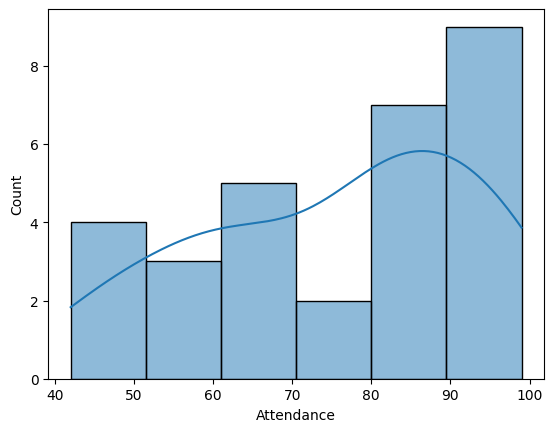
\includegraphics[width=0.75\textwidth]{img/exp6_attendanceHist.png}
    % \caption{Marks of Each Student — Bar Chart}
    % \label{fig:marks_bar}
\end{figure}

\subsection{Observation}

i. The Marks distribution is left skewed and loaded towards 85-95 range. The curve not forming a symmetric bell shape.

ii. The StudyHours distribution is the closest to normal among the three. The curve is roughtly bell-shaped and centered. The spike at 6-7 hours prevents it from being perfect.

iii. The Attendance distribution mirrors the Marks distribution. 

iv. Overall, none of the three variable follow a perfect normal distribution. Marks and Attendance are left-skewed, while StudyHour would have been perfect if there was no spike at 6-7 hours.

